% \documentclass[aspectratio=169,notes]{beamer}
\documentclass[aspectratio=169]{beamer}
\usetheme[faculty=phil]{fibeamer}
\usepackage{polyglossia}
\setmainlanguage{english} %% main locale instead of `english`, you
%% can typeset the presentation in either Czech or Slovak,
%% respectively.
\setotherlanguages{russian} %% The additional keys allow
%%
%%   \begin{otherlanguage}{czech}   ... \end{otherlanguage}
%%   \begin{otherlanguage}{slovak}  ... \end{otherlanguage}
%%
%% These macros specify information about the presentation
\title[AGLA1]{Analytical Geometry and Linear Algebra I, Lab 11} %% that will be typeset on the
\subtitle{Affine Transformation
\\ \   \\ \ 
         } %% title page.
\author{Oleg Bulichev}
%% These additional packages are used within the document:
\usepackage{ragged2e}  % `\justifying` text
\usepackage{booktabs}  % Tables
\usepackage{tabularx}
\usepackage{tikz}      % Diagrams
\usetikzlibrary{calc, shapes, backgrounds}
\usepackage{amsmath, amssymb}
\usepackage{url}       % `\url`s
\usepackage{listings}  % Code listings
% \usepackage{subfigure}
\usepackage{floatrow}
\usepackage{subcaption}
\usepackage{mathtools}
\usepackage{todonotes}
\usepackage{fontspec}
\usepackage{multicol}
\usepackage{pdfpages}
\usepackage{wrapfig}
\usepackage{animate}
\usepackage{booktabs}
\usepackage{multirow}

\graphicspath{{resources/}}
\frenchspacing

\setbeamertemplate{caption}[numbered]
\usetikzlibrary{graphs}

% \usepackage[backend=biber,style=ieee,autocite=footnote]{biblatex}
% \addbibresource{biblio.bib}
% \DefineBibliographyStrings{english}{%
%   bibliography = {References},}

\newcommand{\oleg}[2][] {\todo[color=red, #1] {OLEG:\\ #2}}
\newcommand{\fbckg}[1]{\usebackgroundtemplate{\includegraphics[width=\paperwidth]{#1}}}%frame background

\usepackage[framemethod=TikZ]{mdframed}
\newcommand{\dbox}[1]{
\begin{mdframed}[roundcorner=3pt, backgroundcolor=yellow, linewidth=0]
\vspace{1mm}
{#1}
\vspace{1mm}
\end{mdframed}
}

\begin{document}
\setlength{\abovedisplayskip}{0pt}
\setlength{\belowdisplayskip}{0pt}
\setlength{\abovedisplayshortskip}{0pt}
\setlength{\belowdisplayshortskip}{0pt}

\fbckg{fibeamer/figs/title_page.png}
\frame[c]{\setcounter{framenumber}{0}
    \usebeamerfont{title}%
    \usebeamercolor[fg]{title}%
    \begin{minipage}[b][6.5\baselineskip][b]{\textwidth}%
        \textcolor{black}{\raggedright\inserttitle}
    \end{minipage}
    % \vskip-1.5\baselineskip

    \usebeamerfont{subtitle}%
    \usebeamercolor[fg]{framesubtitle}%
    \begin{minipage}[b][3\baselineskip][b]{\textwidth}
        \raggedright%
        \insertsubtitle%
    \end{minipage}
    \vskip.25\baselineskip
}
%   \frame[c]{\maketitle}

\fbckg{fibeamer/figs/common.png}

\note{Решения к ответам лежат в отдельной папке}
% \begin{frame}[t]{Questions for today}
%     \framesubtitle{}
%     \begin{itemize}
%         \item How can I work with general form of 2nd order curve equation?
%         \item How it relates with cone?
%         \item What forms of equation do we have?
%     \end{itemize}
% \end{frame}

\begin{frame}[t]{Affine Transformation}
\framesubtitle{Formal definition}
    
\end{frame}

\begin{frame}[t]{Affine Transformation}
    \framesubtitle{Video: formal definition}
    \vspace{-0.6cm}
    \begin{figure}[H]
        \href{https://www.youtube.com/watch?v=il6Z5LCykZk}{
            \centering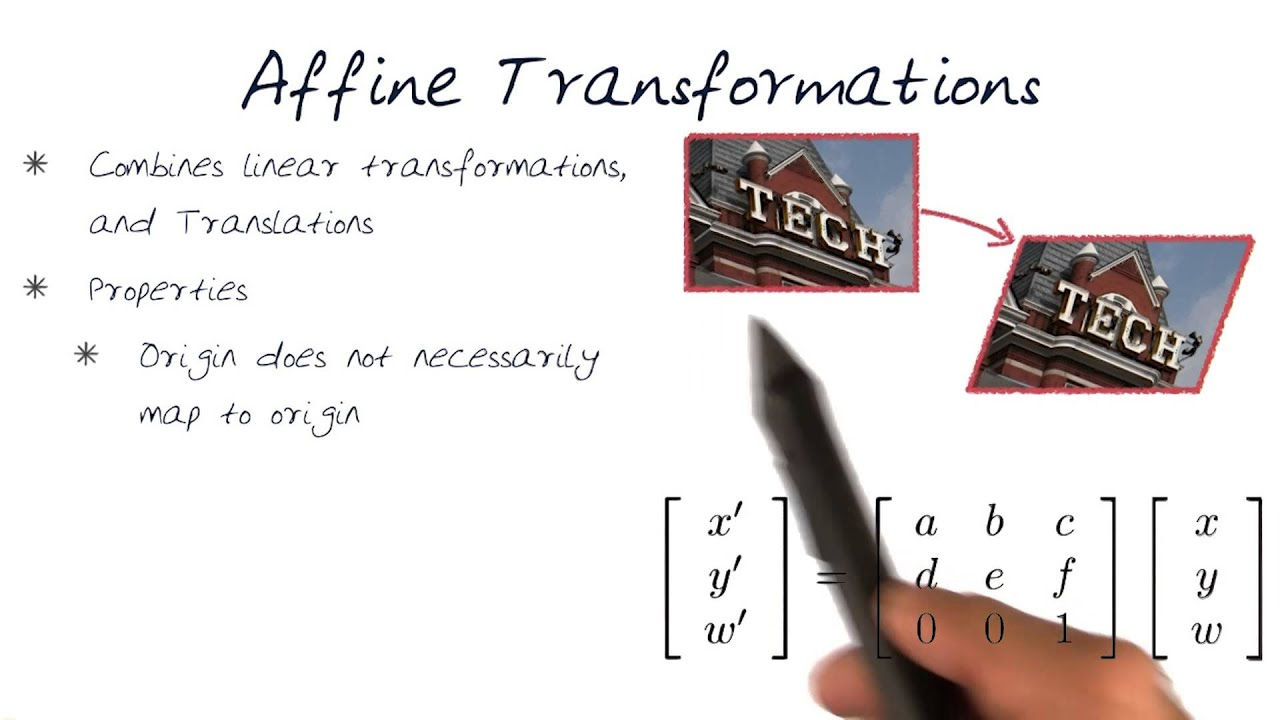
\includegraphics[height=6cm,width=1\textwidth,keepaspectratio]{formal_def.jpg}}
        % \caption{Click on a picture for a video}
        \label{fig:formal_def.jpg}
    \end{figure}
\end{frame}

\begin{frame}[t]{Task 1}
    \framesubtitle{}
    Linear transformation of a real axis is given by $f(x)=ax+b$. (a) Find all fixed points of this transformation. (b) Find the transformation that is inverse for $f$.

    \uncover<2->{
        \alert{\Large Answer}

        (a) If $a\neq1$ then there is one fixed point $x=\frac b{1-a}$; if $a=1$ and $b=0$ then all points are fixed; if $a=1$ and $b\neq0$ then there are no fixed points. (b) It exists only if $a\neq0$: $f^{-1}(y)=\frac{y-b}a$.
    }
\end{frame}

\begin{frame}[t]{Task 2}
    \framesubtitle{}
    An affine transformation is given by $x*=3x+2y-6$, $y*=4x-3y+1$. Find the images of (a) point $M(-1;\,5)$; (b) line $2x+3y=7$.

    \uncover<2->{
        \alert{\Large Answer}

        (a) $(1;-18)$\\ (b) $18x-5y-6=0$.
    }
\end{frame}


\begin{frame}[t]{Affine Transformation}
\framesubtitle{Porperties}
    \begin{itemize}
        \item collinearity between points: three or more points which lie on the same line (called collinear points) continue to be collinear after the transformation.
        \item parallelism: two or more lines which are parallel, continue to be parallel after the transformation.
        \item convexity of sets: a convex set continues to be convex after the transformation. Moreover, the extreme points of the original set are mapped to the extreme points of the transformed set.
        \item ratios of lengths of parallel line segments
    \end{itemize}
\end{frame}

\begin{frame}[t]{Task 3}
    \framesubtitle{}
    Two linear transformations of a real axis $f$ and $g$ are given by $f(x)=ax+b$, $g(x)=cx+d$. Find compositions of transformations $fg$ and $gf$. What are the necessary and sufficient conditions for $fg$ to be equal to $gf$?
    
    \uncover<2->{
        \alert{\Large Answer}
        
        $(fg)(x)=acx+ad+b$; $(gf)(x)=acx+bc+d$; $fg=gf\Leftrightarrow d(a-1)=b(c-1)$.
    }
\end{frame}

\begin{frame}[t]{Bijection, injection and surjection}
\framesubtitle{}
    \vspace{-0.6cm}
    \begin{figure}[H]
        \centering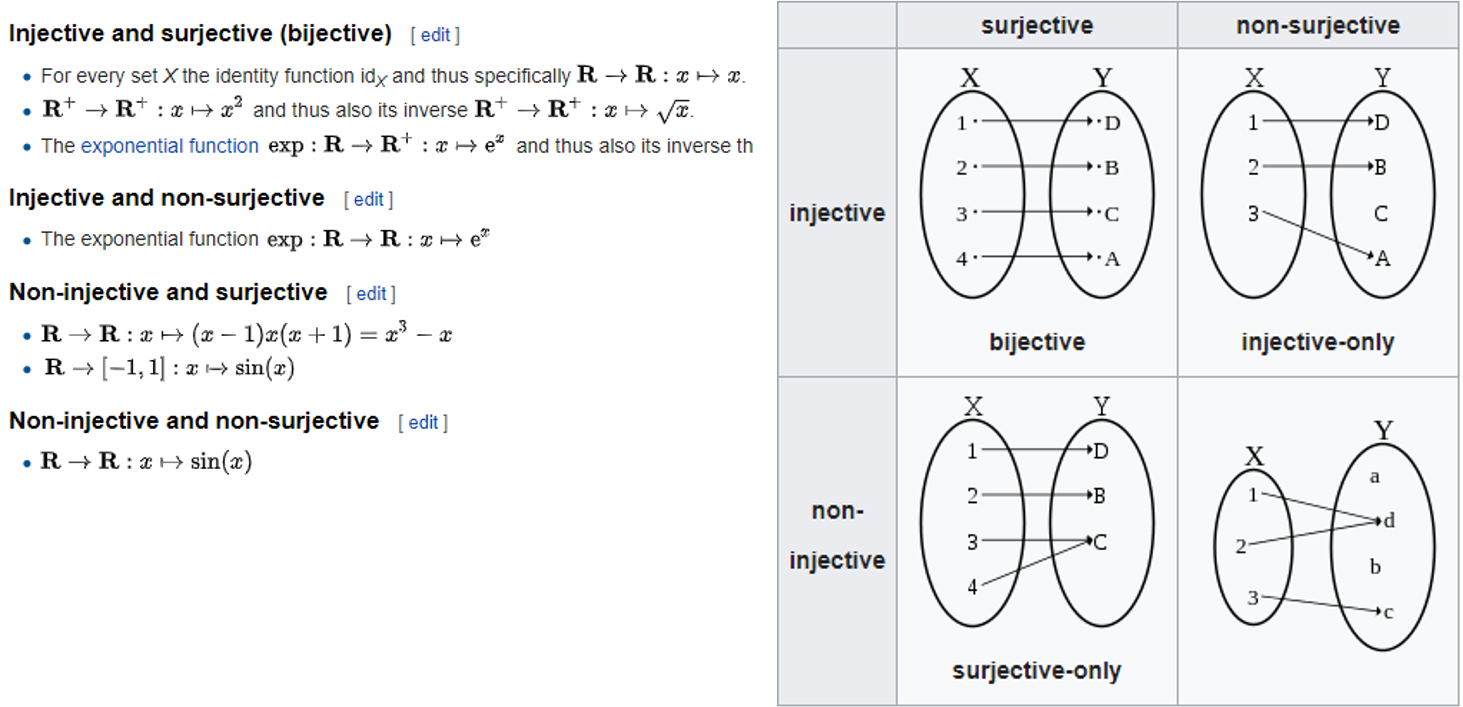
\includegraphics[height=6.5cm,width=1\textwidth,keepaspectratio]{bij_inj_surj_full.png}
        \label{fig:bij_inj_surj_full.png}
    \end{figure}
\end{frame}

% \begin{frame}[t]{Bijection, injection and surjection}
% \framesubtitle{Definition}
% \vspace{-0.5cm}
%     \begin{columns}[T,onlytextwidth]
%         \scriptsize
%         \begin{column}{0.59\textwidth}
%             \textbf{Injective}: \\
%             A function is injective (one-to-one) if each possible element of the codomain is mapped to by at most one argument. Equivalently, a function is injective if it maps distinct arguments to distinct images.

% The function {\displaystyle f\colon X\to Y}f \colon X \to Y is injective, if for all {\displaystyle x,x'\in X}{\displaystyle x,x'\in X}, {\displaystyle f(x)=f(x')\Rightarrow x=x'.}{\displaystyle f(x)=f(x')\Rightarrow x=x'.}

% \textbf{Surjection}: \\ 
% A function is surjective or onto if each element of the codomain is mapped to by at least one element of the domain. In other words, each element of the codomain has non-empty preimage. Equivalently, a function is surjective if its image is equal to its codomain.

% The function {\displaystyle f\colon X\to Y}f \colon X \to Y is surjective, if for all {\displaystyle y\in Y}y\in Y, there is {\displaystyle x\in X}x\in X such that {\displaystyle f(x)=y.}{\displaystyle f(x)=y.}

% \textbf{Bijection}: \\ 
% A function is bijective if it is both injective and surjective. A bijective function is also called a bijection or a one-to-one correspondence. A function is bijective if and only if every possible image is mapped to by exactly one argument.

% The function {\displaystyle f\colon X\to Y}f \colon X \to Y is bijective, if for all {\displaystyle y\in Y}y\in Y, there is a unique {\displaystyle x\in X}x\in X such that {\displaystyle f(x)=y.}{\displaystyle f(x)=y.}

%         \end{column}
%         \begin{column}{0.39\textwidth}
%             \begin{figure}[H]
%                 \centering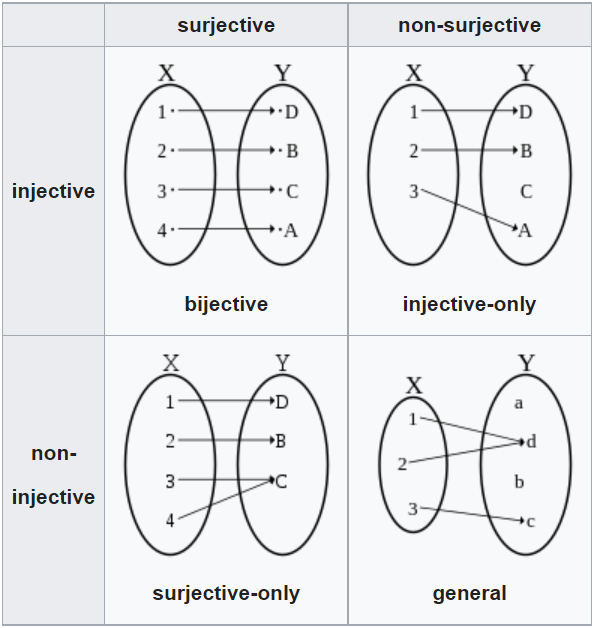
\includegraphics[height=4cm,width=1\textwidth,keepaspectratio]{bij_inj_surj.png}
%                 % \caption{caption_name}
%                 \label{fig:bij_inj_surj.png}
%             \end{figure}
%         \end{column}
%     \end{columns}
% \end{frame}

% \begin{frame}[t]{}
% \framesubtitle{Examples}
% \textbf{Injective and surjective (bijective)}
% The identity function idX for every non-empty set X, and thus specifically {\displaystyle \mathbf {R} \to \mathbf {R} :x\mapsto x.}{\displaystyle \mathbf {R} \to \mathbf {R} :x\mapsto x.}
% {\displaystyle \mathbf {R} ^{+}\to \mathbf {R} ^{+}:x\mapsto x^{2}}{\displaystyle \mathbf {R} ^{+}\to \mathbf {R} ^{+}:x\mapsto x^{2}}, and thus also its inverse {\displaystyle \mathbf {R} ^{+}\to \mathbf {R} ^{+}:x\mapsto {\sqrt {x}}.}{\displaystyle \mathbf {R} ^{+}\to \mathbf {R} ^{+}:x\mapsto {\sqrt {x}}.}
% The exponential function {\displaystyle \exp \colon \mathbf {R} \to \mathbf {R} ^{+}:x\mapsto \mathrm {e} ^{x}}{\displaystyle \exp \colon \mathbf {R} \to \mathbf {R} ^{+}:x\mapsto \mathrm {e} ^{x}} (that is, the exponential function with its codomain restricted to its image), and thus also its inverse the natural logarithm {\displaystyle \ln \colon \mathbf {R} ^{+}\to \mathbf {R} :x\mapsto \ln {x}.}{\displaystyle \ln \colon \mathbf {R} ^{+}\to \mathbf {R} :x\mapsto \ln {x}.}

% \textbf{Injective and non-surjective}
% The exponential function {\displaystyle \exp \colon \mathbf {R} \to \mathbf {R} :x\mapsto \mathrm {e} ^{x}.}{\displaystyle \exp \colon \mathbf {R} \to \mathbf {R} :x\mapsto \mathrm {e} ^{x}.}

% \textbf{Non-injective and surjective}
% {\displaystyle \mathbf {R} \to \mathbf {R} :x\mapsto (x-1)x(x+1)=x^{3}-x.}{\displaystyle \mathbf {R} \to \mathbf {R} :x\mapsto (x-1)x(x+1)=x^{3}-x.}
% {\displaystyle \mathbf {R} \to [-1,1]:x\mapsto \sin(x).}{\displaystyle \mathbf {R} \to [-1,1]:x\mapsto \sin(x).}

% \textbf{Non-injective and non-surjective}
% {\displaystyle \mathbf {R} \to \mathbf {R} :x\mapsto \sin(x).}{\displaystyle \mathbf {R} \to \mathbf {R} :x\mapsto \sin(x).}
% \end{frame}

\begin{frame}[t]{Task 4}
    \framesubtitle{}
    \only<1>{
        Transformation of a plane is given by $x*=x^2-y^2$, $y*=2xy$. Is this transformation an (a) injection; (b) surjection; (c) bijection? (d) Find the preimage of point $(x*;y*)$ by this transformation.
        }
    \only<2>{
        \alert{\Large Answer}
        
        (a): Not Injection \\ 
        (b): Is surjection \\ 
        (c): Not Bijection
    }
\end{frame}

\begin{frame}[t]{Affine Transformation}
\framesubtitle{In Computer Vision (CV)}
    \vspace{-0.6cm}
    \begin{figure}[H]
        \centering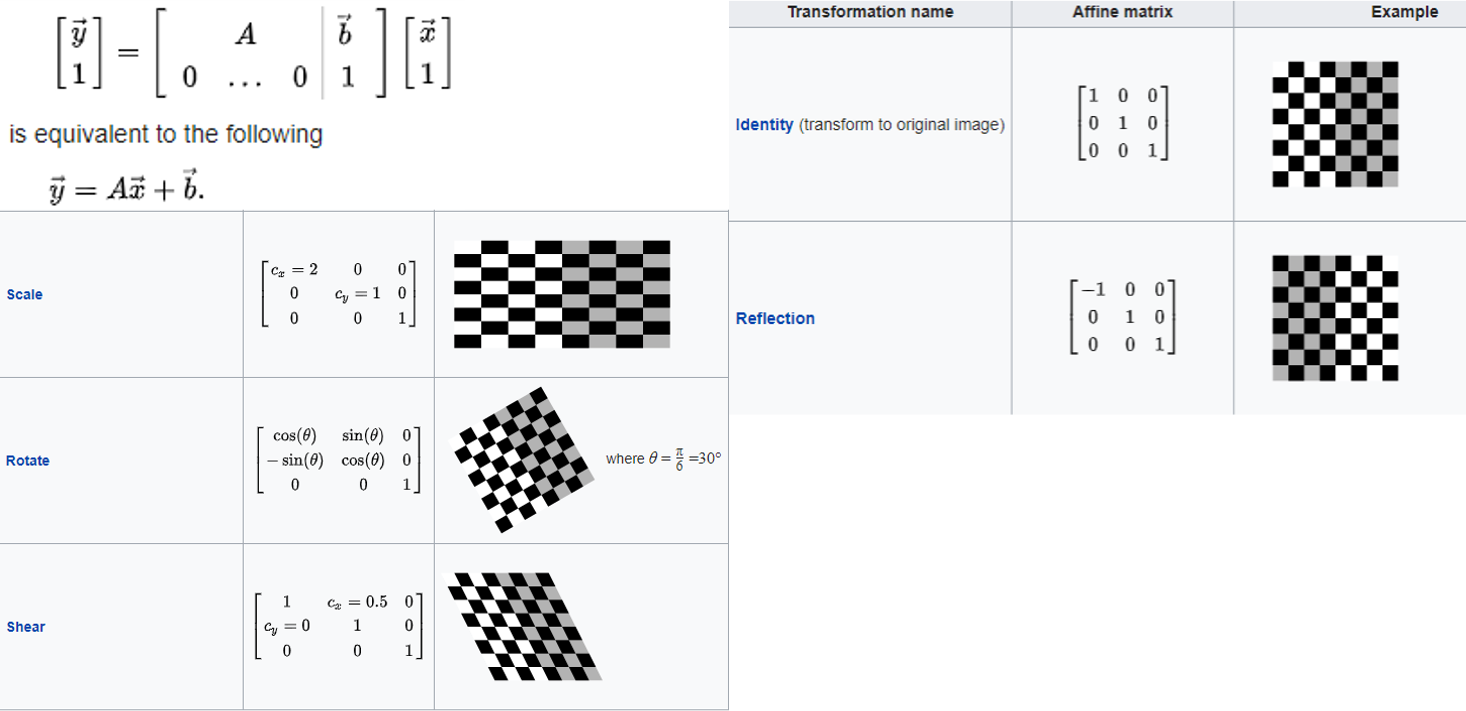
\includegraphics[height=6cm,width=1\textwidth,keepaspectratio]{affine_cv.png}
        \label{fig:affine_cv.png}
    \end{figure}
\end{frame}

\begin{frame}[t]{Affine Transformation}
    \framesubtitle{Video: intuition besides numbers 2D}
    \vspace{-0.6cm}
    \begin{figure}[H]
        \href{https://youtu.be/Y_TKQKdWC2k}{
            \centering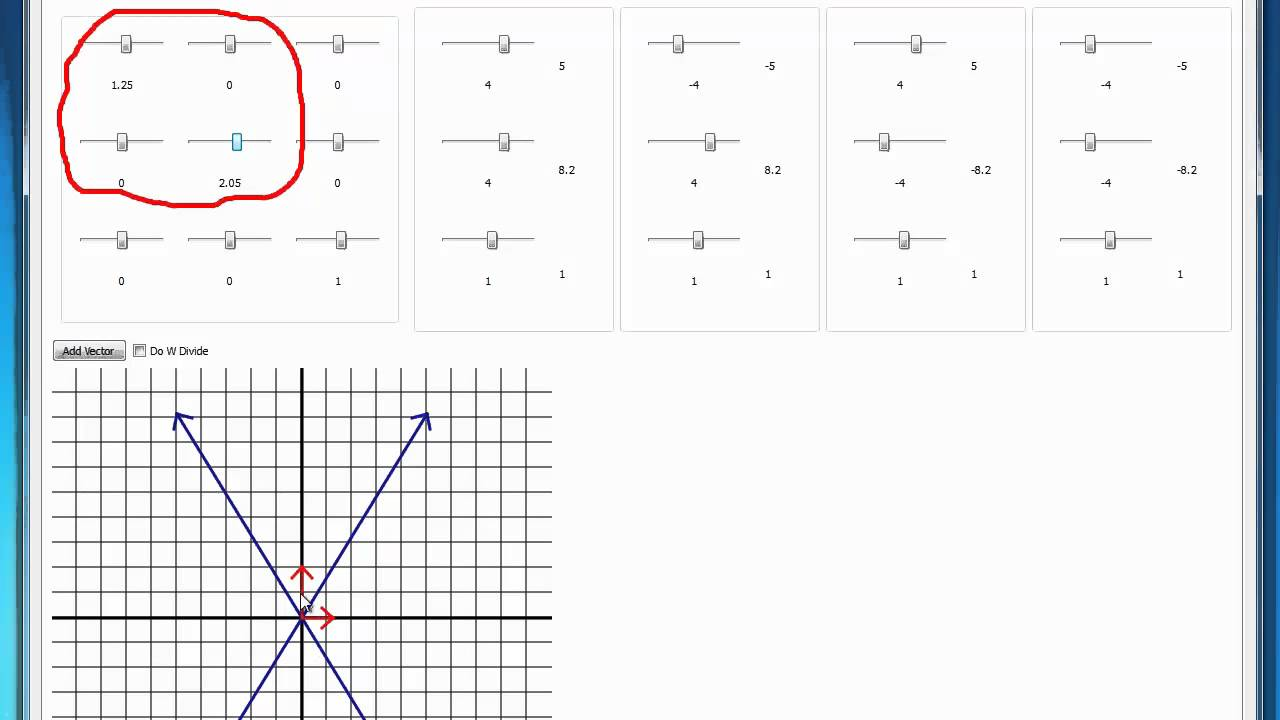
\includegraphics[height=6cm,width=1\textwidth,keepaspectratio]{num_intuition.jpg}}
        % \caption{Click on a picture for a video}
        \label{fig:num_intuition.jpg}
    \end{figure}
\end{frame}

\begin{frame}[t]{Affine Transformation}
    \framesubtitle{Video}
    \vspace{-0.6cm}
    \begin{figure}[H]
        \href{https://youtu.be/E3Phj6J287o}{
            \centering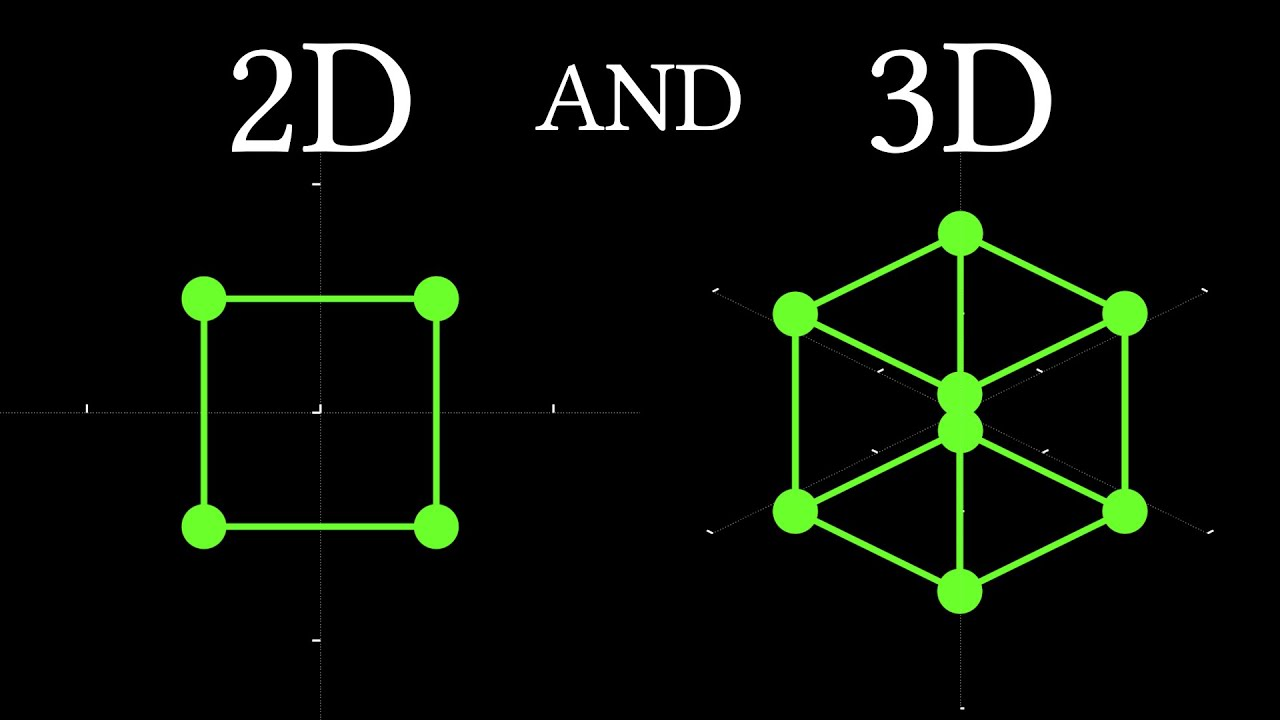
\includegraphics[height=6cm,width=1\textwidth,keepaspectratio]{num_intuition_3d.jpg}}
        % \caption{Click on a picture for a video}
        \label{fig:num_intuition_3d.jpg}
    \end{figure}
\end{frame}

\begin{frame}[t]{Affine Transformation}
    \framesubtitle{Application in CV (1)}
        \vspace{-0.6cm}
        \begin{figure}[H]
            \centering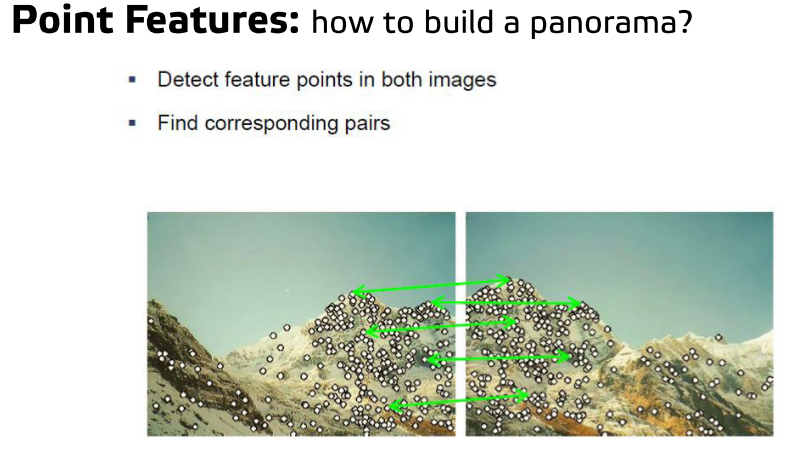
\includegraphics[height=6cm,width=1\textwidth,keepaspectratio]{cv_intro.png}
            \label{fig:cv_intro.png}
        \end{figure}
    \end{frame}

\begin{frame}[t]{Affine Transformation}
\framesubtitle{Application in CV (2)}
    \vspace{-0.6cm}
    \begin{figure}[H]
        \centering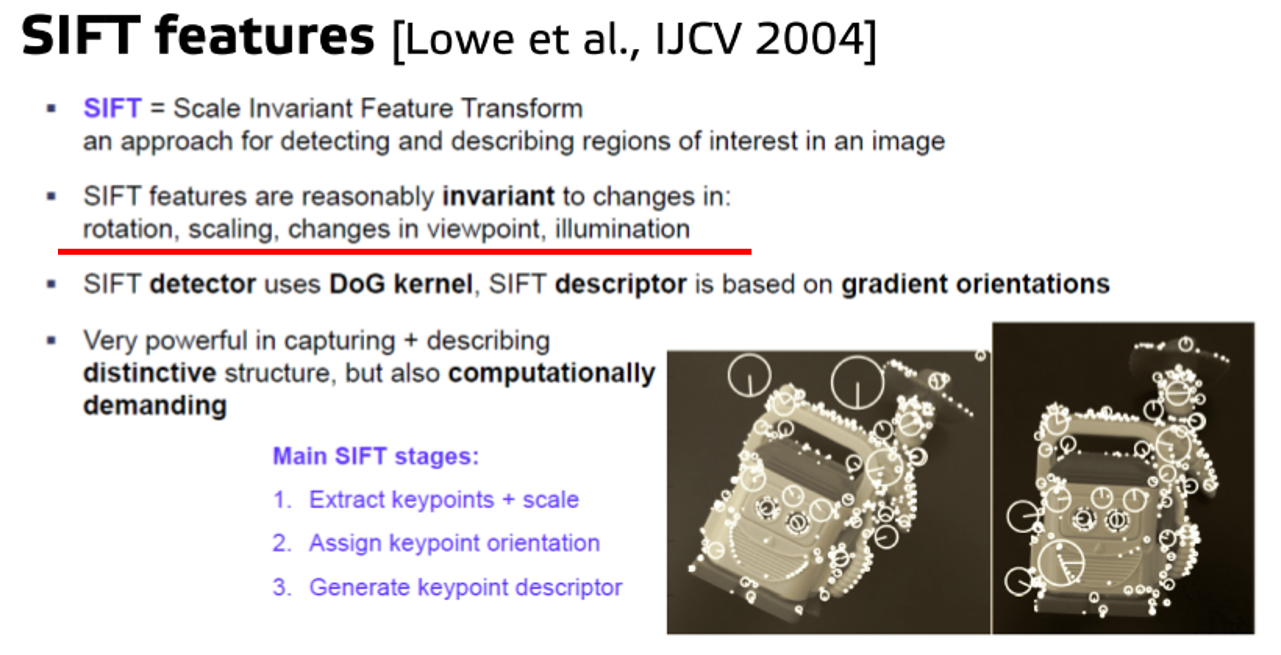
\includegraphics[height=6cm,width=1\textwidth,keepaspectratio]{sift.png}
        \label{fig:sift.png}
    \end{figure}
\end{frame}

\begin{frame}[t]{Affine Transformation}
    \framesubtitle{Application in CV (3)}
        \vspace{-0.6cm}
        \begin{figure}[H]
            \centering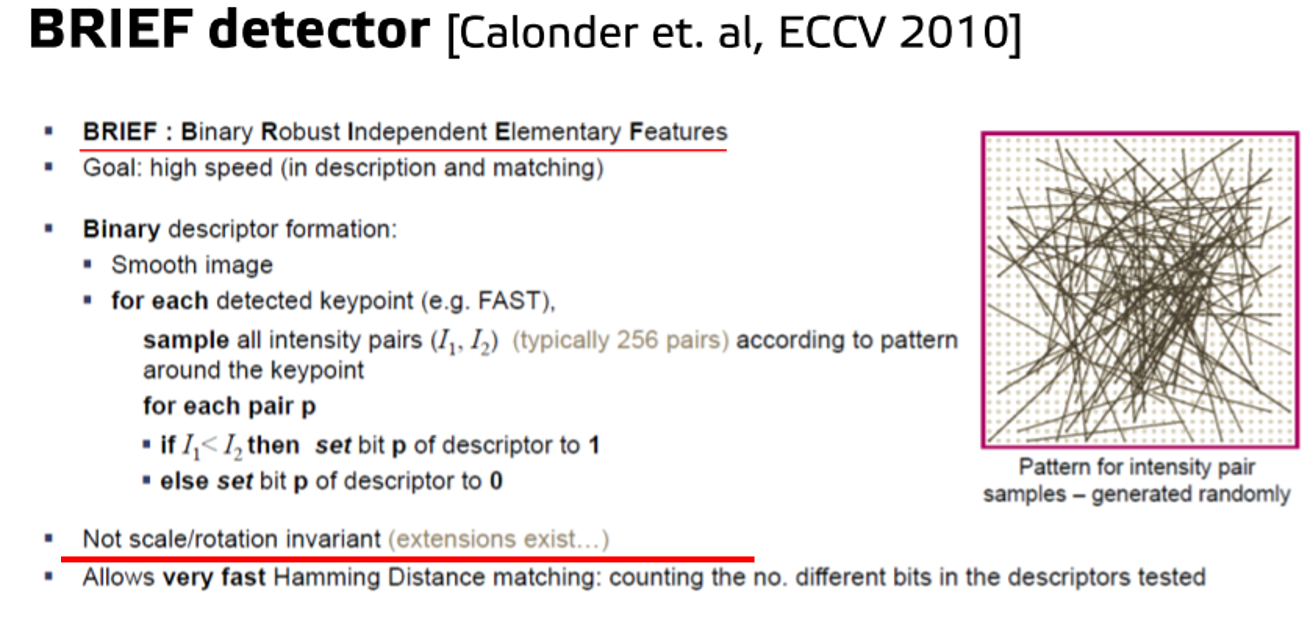
\includegraphics[height=6cm,width=1\textwidth,keepaspectratio]{brief.png}
            \label{fig:brief.png}
        \end{figure}
    \end{frame}

\begin{frame}[t]{Task 5}
    \framesubtitle{}
    \only<1>{
        Find the image of an arbitrary point $M$ which has position vector $\textbf{r}$ by the following transformations:

        (a) homothety with center $M_0(\textbf{r}_0)$ and ratio $\lambda\neq0$;
        
        (b) reflection across point $M_0(\textbf{r}_0)$;
        
        (c) translation by vector $\textbf{a}$;
        
        (d) orthogonal projection onto the line $\textbf{r}=\textbf{r}_0+\textbf{a}t$;
        
        (e) reflection across the line $\textbf{r}=\textbf{r}_0+\textbf{a}t$; 
        
        (f) dilation of factor $\lambda>0$ from the line $\textbf{r}=\textbf{r}_0+\textbf{a}t$.
        }
    \only<2>{
        \alert{\Large Answer}

        (a) $\textbf{r}*=\textbf{r}_0+\lambda(\textbf{r}-\textbf{r}_0)$; 
        
        (b) $\textbf{r}*=-\textbf{r}+2\textbf{r}_0$; 
        
        (c) $\textbf{r}*=\textbf{r}+\textbf{a}$;
        
        (d) $\textbf{r}*=\textbf{r}_0+\frac{\left(\textbf{r}-\textbf{r}_0\right)\cdot\textbf{a}}{|\textbf{a}|^2}\textbf{a}$; 
        
        (e) $\textbf{r}*=2\textbf{r}_0-\textbf{r}+2\frac{\left(\textbf{r}-\textbf{r}_0\right)\cdot\textbf{a}}{|\textbf{a}|^2}\textbf{a}$;
        
        (f) $\textbf{r}*=\lambda\textbf{r}+(1-\lambda)\textbf{r}_0+(1-\lambda) \frac{\left(\textbf{r}-\textbf{r}_0\right)\cdot\textbf{a}}{|\textbf{a}|^2}\textbf{a}$.
    }
\end{frame}

\begin{frame}[t]{Task 6}
    \framesubtitle{}
    \only<1>{
        Find formulas for the following affine transformations:

        (a) orthogonal projection onto line $x-3y+1=0$;
        
        (b) reflection across line $3x+4y-1=0$;
        
        (c) dilation from line $x+y-2=0$ of factor $\frac13$;
        
        (d) dilation from line $2x-y+5=0$ of factor 2.  
    }
    \only<2>{
        \alert{\Large Answer}

        (a) $x^*=\frac{9x+3y-1}{10}$, $y^*=\frac{3x+y+3}{10}$; 
        
        (b) $x^*=\frac{7x-24y+6}{25}$, $y^*={-24x-7y+8}{25}$; 
        
        (c) $x^*=\frac{2x-y+2}3$, $y^*=\frac{-x+2y+2}3$; 
        
        (d) $x^*=\frac{9x-2y+10}5$, $y^*=\frac{-2x+6y-5}5$.
    }
\end{frame}

\begin{frame}[t]{Task 7}
    \framesubtitle{}
    \only<1>{
    Find formulas for an affine mapping that transforms

(a) points $A(\frac37;\,1)$, $B(1;\frac14)$, $C(2;-1)$ into points $A*(-4;\,2)$, $B*(-1;\,6)$, $C*(4;\,13)$ respectively;

(b) points $A(0;\,0)$, $B(-1;\,2)$, $C(1;-2)$ into points $A*(-1;-1)$, $B*(0;\,0)$, $C*(1;\,1)$ respectively;

(c) points $A(2;\,0)$, $B(3;-1)$, $C(4;-2)$ into points $A*(2;\,1)$, $B*(-2;-1)$, $C*(-6;-3)$ respectively;

(d) points $A(-2;\,0)$, $B(2;-1)$, $C(0;\,4)$ into points $A*(-2;\,1)$, $B*(2;\,1)$, $C*(0;\,1)$ respectively.}
    \only<2>{
        \alert{\Large Answer}

        (a) $x*=-4y$, $y*=7x-1$; 
        
        (b) no solutions; 
        
        (c) $x*=px+(p+4)y+2-2p$, $y*=qx+(q+2)y+1-2q$, where $p$ and $q$ are any real numbers; 
        
        (d) no solutions (there exists a linear transformation that is not affine).
    }
\end{frame}

\begin{frame}[t]{Task 8}
    \framesubtitle{}
    Find all invariant lines of an affine transformation given by

(a) $x*=y$, $y*=1-x$;

(b) $x*=2x+y-3$, $y*=-3x-y$;

(c) $x*=5x+3y+1$, $y*=-3x-y$.

    \uncover<2->{
        \alert{\Large Answer}

        (a) no solutions; 
        
        (b) $x+y-3=0$, $2x-y+p=0$, where $p$ can be any real number; 
        
        (c) $x+y+1=0$.
    }
\end{frame}




\begin{frame}[t]{Reference material}
    % \framesubtitle{OnlineMschool}
    \Large
    \begin{itemize}
        \item \href{https://en.wikipedia.org/wiki/Bijection,_injection_and_surjection}{Bijection, injection and surjection (wiki)}
        \item \href{https://en.wikipedia.org/wiki/Affine_transformation}{Affine transformation (wiki)}
    \end{itemize}
\end{frame}

\fbckg{fibeamer/figs/last_page.png}
\frame[plain]{}

\end{document}